%!TEX TS-program = xelatex
\documentclass[]{friggeri-cv}
\usepackage{graphicx}
\addbibresource{bibliography.bib}

\begin{document}
\header{adrien}{friggeri}
       {social network analyst}


% In the aside, each new line forces a line break
\begin{aside}
    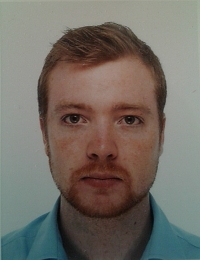
\includegraphics[width=100pt]{photo.png}
  \section{about}
    31 rue Smith
    69002 Lyon
    France
    ~
    \href{mailto:adrien@friggeri.net}{adrien@friggeri.net}
    \href{http://friggeri.net}{http://friggeri.net}
    \href{http://facebook.com/adrien}{fb://adrien}
  \section{languages}
    bilingual french/english
    spanish \& italian notions
  \section{programming}
    {\color{red} $\varheartsuit$} JavaScript
    (ES5, node.js)
    Python, C, OCaml
    CSS3 \& HTML5
\end{aside}

\section{interests}

complex networks, social networks, community detection, community structure,
overlapping communities, information diffusion, viral marketing, social
inference, recommendation, data mining

\section{education}

\begin{entrylist}
  \entry
    {since 2009}
    {Ph.D. {\normalfont candidate in Computer Science}}
    {DNET/INRIA, LIP/ÉNS de Lyon}
    {\emph{A Quantified Theory of Social Cohesion.}}
  \entry
    {2007–2008}
    {M.Sc. magna cum laude}
    {IXXI, École Normale Supérieure de Lyon}
    {Majoring in Computer Science\\
    Specialization in Complex Systems}
  \entry
    {2006–2007}
    {B.Sc. magna cum laude}
    {École Normale Supérieure de Lyon}
    {Majoring in Computer Science}
  \entry
    {2003–2006}
    {Classes Préparatoires aux Grandes Écoles}
    {Lycée Fénelon, Lycée Louis le Grand, Paris}
    {Preparation for national competitive entrance exams to leading French ``grandes écoles'', specializing in mathematics and physics.}
  \entry
    {2003}
    {French Baccalauréat S. with honors}
    {Lycée Louis le Grand, Paris}
    {Specialization in mathematics and physics}
\end{entrylist}

\section{experience}

\begin{entrylist}
  \entry
    {02–07 2009}
    {LIP6/CNRS, Paris}
    {Research Internship.}
    {\emph{Visualization of complex networks.}}
  \entry
    {06–08 2008}
    {ISCPIF/CNRS, Paris}
    {Research Internship.}
    {\emph{Diffusion in the Blogosphere. Happy Flu.}}
  \entry
    {06–08 2007}
    {LIP6/CNRS, Paris}
    {Research Internship.}
    {\emph{Kernels in real world networks.}}
  \entry
    {07–08 2005}
    {\href{http://www.kelkoo.com}{Kelkoo.com}}
    {Summer job.}
    {\emph{Creation of a keyword generator for Google Adwords.}}
  \entry
    {07–08 2004}
    {\href{http://www.monsieurprix.com}{MonsieurPrix.com}}
    {Summer job.}
    {\emph{Development of an e-commerce product indexation spider.}}
\end{entrylist}

\section{applications}

\begin{entrylist}
  \entry
    {2012}
    {Who did I forget ?}
    {\href{http://whodidiforget.com}{whodidiforget.com}}
    {Guest list recommendation for Facebook events based on friends already attending the event.}
  \entry
    {2011}
    {Fellows}
    {\href{http://fellows-exp.com}{fellows-exp.com}}
    {Automatic community detection among Facebook Friends in order to validate the \emph{cohesion} measure, creation of friend lists.}
  \entry
    {2008}
    {Happy Flu}
    {\href{http://happyflu.com}{happyflu.com}}
    {Experiment aimed to measure viral spreading of content across the blogosphere.}
\end{entrylist}

\section{publications}


\printbibsection{article}{article in peer-reviewed journal}
\begin{refsection}
  \nocite{*}
  \printbibliography[sorting=chronological, type=inproceedings, title={international peer-reviewed conferences/proceedings}, notkeyword={france}, heading=subbibliography]
\end{refsection}
\begin{refsection}
  \nocite{*}
  \printbibliography[sorting=chronological, type=inproceedings, title={local peer-reviewed conferences/proceedings}, keyword={france}, heading=subbibliography]
\end{refsection}
\printbibsection{misc}{other publications}
\printbibsection{report}{research reports}

\end{document}
